	\documentclass{article}
			
		\usepackage{parskip}
		\usepackage{listings}
		\usepackage{xcolor}
		\usepackage{textcomp}
			
		%STYLE AND COLOR DEFINITION FOR SOURCE CODE 	
		\newcommand{\PHPamountofcolor}{75}
		\newcommand{\SourceCodeContext}{5}
		%Lets define the php language colors:
		\definecolor{PHP_comment_old}{HTML}{FF8000}
		\colorlet{PHP_comment}{PHP_comment_old!\PHPamountofcolor!black}
		\definecolor{PHP_default_old}{HTML}{000000}
		\colorlet{PHP_default}{PHP_default_old!\PHPamountofcolor!black}
		\definecolor{PHP_keyword_old}{HTML}{6c9c11}
		\colorlet{PHP_keyword}{PHP_keyword_old!\PHPamountofcolor!black}
		\definecolor{PHP_emph1_old}{HTML}{0F58A2}
		\colorlet{PHP_emph1}{PHP_emph1_old!\PHPamountofcolor!black}
		\definecolor{PHP_emph2_old}{HTML}{CCAA00}
		\colorlet{PHP_emph2}{PHP_emph2_old!\PHPamountofcolor!black}
		\definecolor{PHP_emph4_old}{HTML}{C60484}
		\colorlet{PHP_emph4}{PHP_emph4_old!\PHPamountofcolor!black}
		\definecolor{PHP_string_old}{HTML}{C78F0A}
		\colorlet{PHP_string}{PHP_string_old!\PHPamountofcolor!black}
		\definecolor{PHP_variable_old}{HTML}{C82210}%C82210
		\colorlet{PHP_variable}{PHP_variable_old!\PHPamountofcolor!black}
		\definecolor{PHP_number_old}{HTML}{BF1CA6}
		\colorlet{PHP_number}{PHP_number_old!\PHPamountofcolor!black}
		%Now we want to highlight the variables. This will be done by triggering the function \PHPhighlightvar at the start of any $ run. This function wil only highlight variables and any other identifiers will be ignored. Luckily lstlisting will only give correct identifiers so we only will have to check if the previous call was made with a $
		\usepackage{fontspec}
		\setmonofont{Courier}
		%\usepackage[utf8]{inputenc}
		%\usepackage[T1]{fontenc}
		%\usepackage{courier, textcomp}
		\usepackage{etoolbox}
		\newtoggle{InString}{}% Keep track of if we are within a string
		\togglefalse{InString}% Assume not initally in string
		
		\newcommand*{\ColorIfNotInString}[1]{\iftoggle{InString}{#1}{\color{PHP_number}#1}}%

		%helper
		
		\newcommand{\PHPhighlightvar}[1]{\ifnum\theDollarFlag=1 \color{PHP_variable} \fi#1\setcounter{DollarFlag}{0}}
		\newcounter{DollarFlag}
		
		%images
		\usepackage{graphicx}
		\graphicspath{ {images/} }
		\usepackage{wrapfig}
		\usepackage{subcaption}
		
		
			
			
			
		
			
			\title{Machine Learning: First Home Work \\ \bigskip \large  Principal Component Analysis and Na??ve Bayes Classification }

			\author{Edoardo Ghini}
			
			\begin{document}
			
			\textbf{\maketitle}
			\pagenumbering{gobble}
			
			\bigskip\bigskip\bigskip
			\begin{center}
			
\includegraphics[width=0.5\textwidth]{laSapienza}
			\end{center}
			\bigskip\bigskip\bigskip
			\textbf{
			Dipartimento di Ingegneria dell'Università di Roma La Sapienza}
			

			\newpage
			\pagenumbering{roman}
			\tableofcontents
			\newpage
			\pagenumbering{arabic}
			
			
			
			
			
			%SETTING STYLE OF SOURCE CODE
			\lstset{
		  language        = php,
		  basicstyle      = \footnotesize\ttfamily,
		  keywordstyle    = \color{PHP_keyword},
		  stringstyle     = \color{PHP_string!90!black}\toggletrue{InString},
		  %this allows highlighting of variables:
		  literate        =  {\$}{{\iftoggle{InString}{\$}{\setcounter{DollarFlag}{1}\color{PHP_variable}\$\color{PHP_default}}}}1
		%    {"}{{{\ProcessQuote{"}}}}1% Disable coloring within double quotes
		%    {'}{{{\ProcessQuote{'}}}}1% Disable coloring within single quote
		    {0}{{{\ColorIfNotInString{0}}}}1
		    {1}{{{\ColorIfNotInString{1}}}}1
		    {2}{{{\ColorIfNotInString{2}}}}1
		    {3}{{{\ColorIfNotInString{3}}}}1
		    {4}{{{\ColorIfNotInString{4}}}}1
		    {5}{{{\ColorIfNotInString{5}}}}1
		    {6}{{{\ColorIfNotInString{6}}}}1
		    {7}{{{\ColorIfNotInString{7}}}}1
		    {8}{{{\ColorIfNotInString{8}}}}1
		    {9}{{{\ColorIfNotInString{9}}}}1,
		  identifierstyle = \color{PHP_default}\PHPhighlightvar,
		  commentstyle    = \color{PHP_comment}\slshape,
		  emph            =[1]{require_once, require, include_once, include, namespace, use, class, function, new},
		  emphstyle       =[1]\color{PHP_emph1},%\bf,
		  emph            =[2]{echo, empty, isset, array, instanceof},
		  emphstyle       =[2]\color{PHP_emph2},%\bf,
		  emph            =[3]{var, const, abstract, 
		                        protected, private, public,
		                        static, final, extends, implements,
		                        global, if, else, foreach ,for,
		                        endforeach, endif, endfor, elseif,
		                        as},
		  emphstyle       =[3]\color{PHP_keyword},%\bf,
		  emph            =[4]{return, throw, exit, __halt_compiler, continue, break},
		  emphstyle       =[4]\color{PHP_emph4},%\bf,
		  breaklines      = true,
		  captionpos      = b,
		  rulecolor       =\color{black},
		  keywords    ={__halt_compiler,    abstract,   and,    array,
		                    as, break,  callable,   case,   catch,  class,
		                    clone,  const,  continue,   declare,    default,
		                    die,    do, echo,   else,   elseif,
		                    empty,  enddeclare, endfor, endforeach, endif,
		                    endswitch,  endwhile,   eval,   exit,   extends,
		                    final,  finally,    for,    foreach,    function,
		                    global, goto, if,   implements, include,
		                    include_once,   instanceof, insteadof,
		                    interface,  isset, list,    namespace,
		                    new,    or, print, private, protected,  public,
		                    require,    require_once, return,   static,
		                    switch, throw,  trait, try, unset, use, var,
		                    while,  xor,    yield,
		  },
		  numbers=left,
		  stepnumber=1,  
		  numberfirstline=true,
		  numberstyle=\footnotesize,
		  xleftmargin=4.0ex,
		  upquote=true,
		  showlines=true
		  }	
			
			\renewcommand{\lstlistingname}{Code}

			
			\part{Introduction}
			
				\section{Scope}
In the first place, during this experience I tried to analyze a dataset made of a sub set of pictures in which it has been necessary to perform a feature extraction. 
				\section{Objectives}
				Some important concepts to underline will be the impact on the analysis brought from the choice of the feature reduction and also the magnitude of the splitting factor between train and test data.
\newpage
			\part{Development}
				\section{Data loading and feature manipulation}
	At first, I loaded in suitable data structures the features coming from the pixels of the images of the chosen objects.
	After that I standardised and reshaped the matrix in order to obtain an optimal approximation of the original dataset.
	Then , the final dataset manipulation was to apply a principal component analysis to take in consideration the most significative vectors in terms of the variance representation.
	The plots shown above represent different choices of PCA vectors according to the expressive capabilities that are embodied in the components near the first.
	  
					\begin{center}
\begin{figure}
\centering
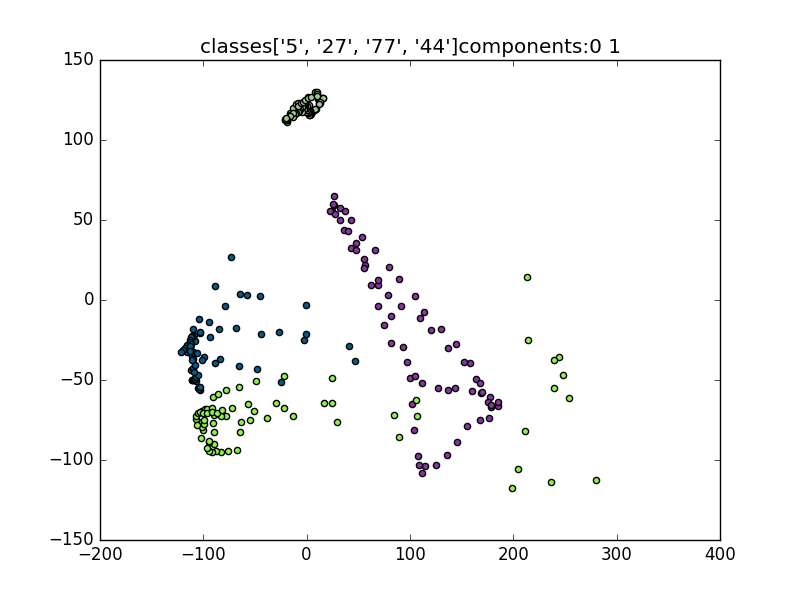
\includegraphics[width=0.9\textwidth]{comp12color}
\caption{}
\label{fig:1}
\end{figure}
\begin{figure}
\centering
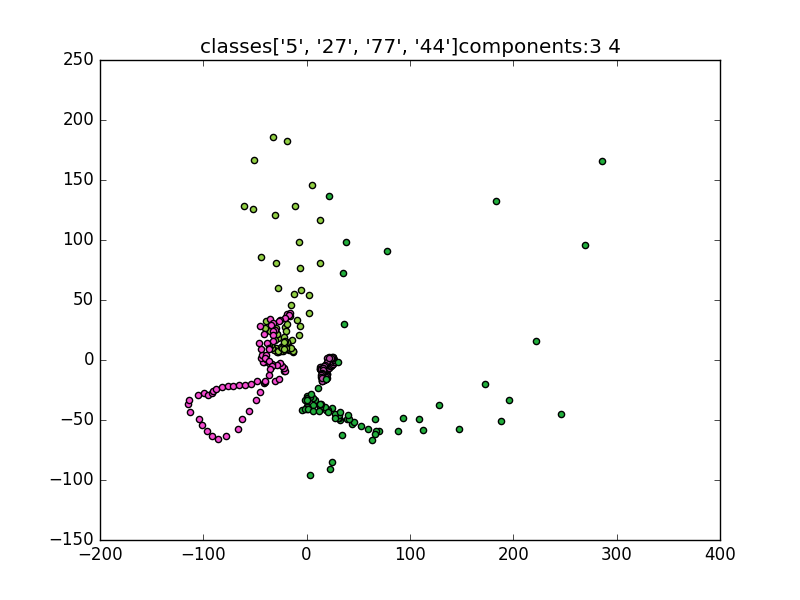
\includegraphics[width=0.9\textwidth]{comp34color}
\caption{}
\label{fig:2}
\end{figure}
\begin{figure}
\centering
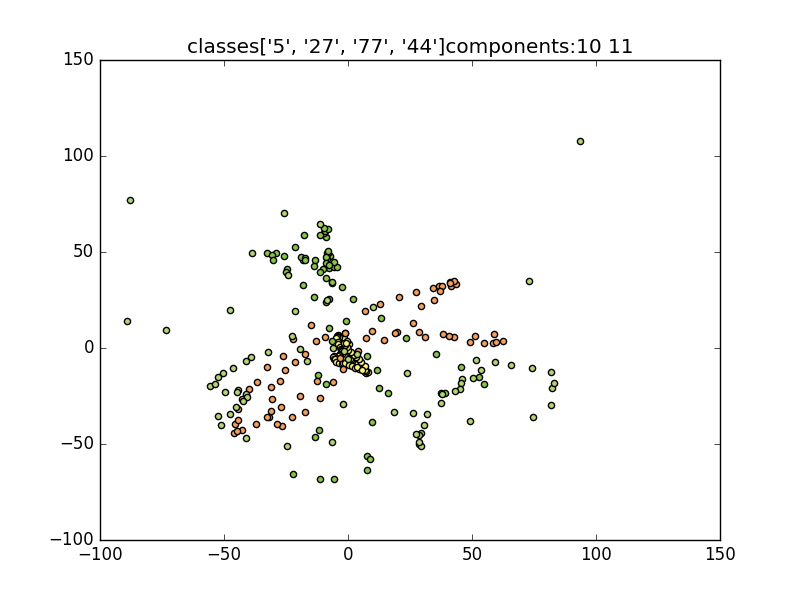
\includegraphics[width=0.9\textwidth]{comp1011}
\caption{}
\label{fig:3}
\end{figure}
\end{center}

As shown in fig.(1) , fig(2 ), and fig(3) there are significative discrepancies between data point concentrations:  in fact, as expected vector choices that are far away from the first principal components gave more vague results.
				\section{Training and Testing}
				\subsection{Data spitting}
				In order to have a feed back on the effectiveness of the model in use, I partitioned my dataset in two subsets. The former will be used to train the model and the latter will be employed to certificate the accuracy of this model. 
				\subsection{Naive Bayes Classification}
				At this point, with a coherent dataset available, I trained a classifier with the subset data chosen to be the prior knowledge for the model. I used a "naive" classifier, a model that works by approximation and in particular it applies a sort of constraint relaxation assuming that all the data vectors where conditionally independent from each others.
				\subsection{Checking model effectiveness}
				Finally I requested a prediction to the trained classifier and I computed a score according to the miss-classification errors encountered.
				Obviously I managed to check the rightness of the predictions thanks to the subset of labels that I have preserved for the test.
				There are some examples below in fig(4), fig(5) and fig(6) that prove that the level of rightness of predictions depends strongly by the rateo chosen to split the subsets of training and testing.
									\begin{center}
\begin{figure}
\centering
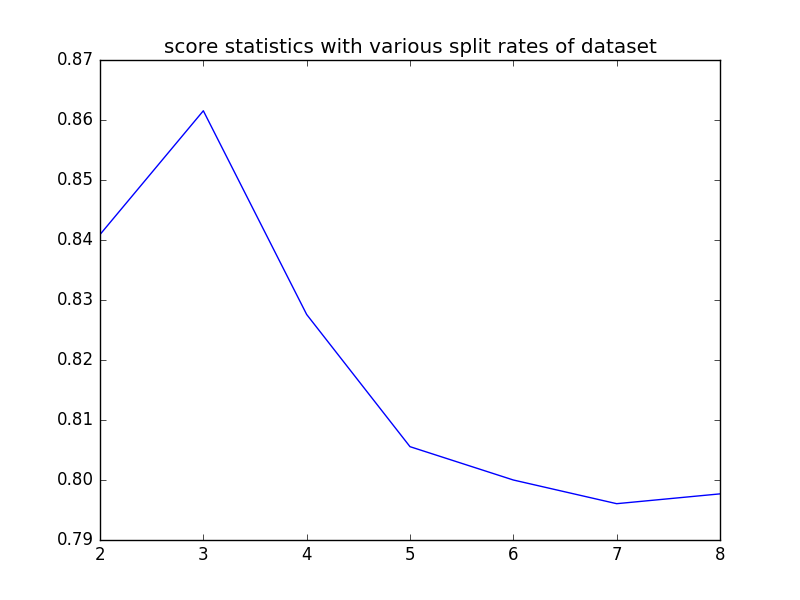
\includegraphics[width=0.9\textwidth]{score-statistics}
\caption{}
\label{fig:4}
\end{figure}
\begin{figure}
\centering
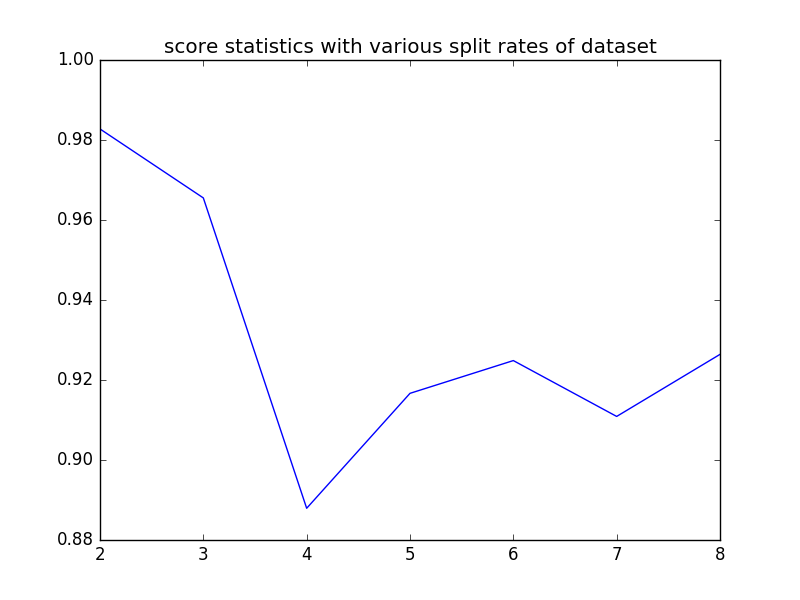
\includegraphics[width=0.9\textwidth]{score-datasplit}
\caption{}
\label{fig:5}
\end{figure}
\begin{figure}
\centering
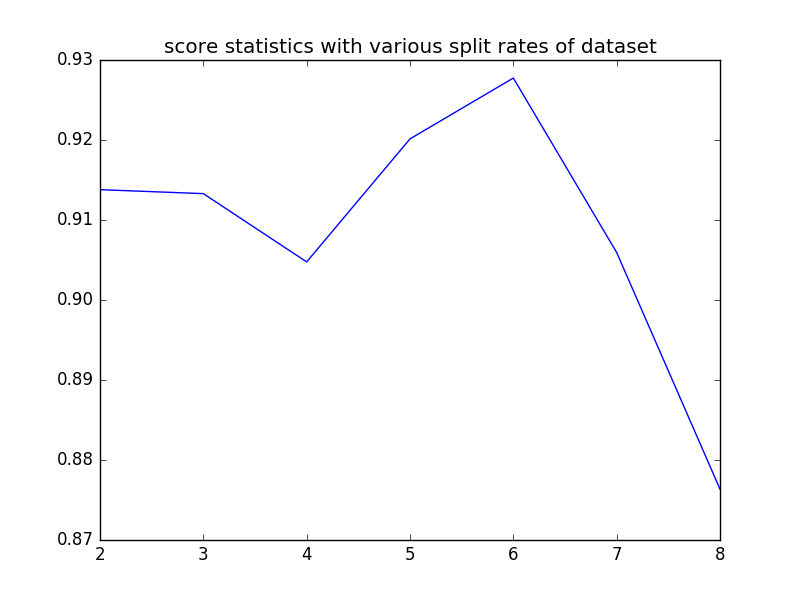
\includegraphics[width=0.9\textwidth]{multiple-classes-score}
\caption{}
\label{fig:6}
\end{figure}
\end{center}

\newpage
			\part{Conclusions}
				
			In conclusion, the difficulties which I would meet with trying to visualize a multidimensional dataset can be mitigated through a feature extraction with a principal component analysis approach.
			However the difficulties in the data representation will grown linearly with the increment of the different classes taken in consideration from the model. For instance in fig(7) there is the case in the dataset representation of much more classes than the aforementioned cases.
			
				
							\begin{center}
\begin{figure}
\centering
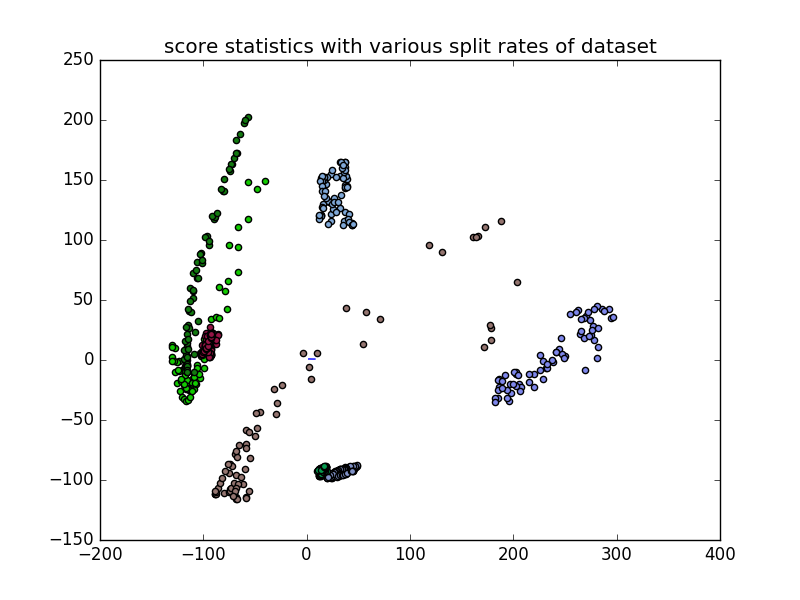
\includegraphics[width=0.9\textwidth]{multiple-classes-dataset}
\caption{}
\label{fig:7}
\end{figure}
\end{center}
		\end{document}
